\documentclass[journal, a4paper]{IEEEtran}
%\author{Huidong Lin}
% some very useful LaTeX packages include:

%\usepackage{cite}      % Written by Donald Arseneau
                        % V1.6 and later of IEEEtran pre-defines the format
                        % of the cite.sty package \cite{} output to follow
                        % that of IEEE. Loading the cite package will
                        % result in citation numbers being automatically
                        % sorted and properly "ranged". i.e.,
                        % [1], [9], [2], [7], [5], [6]
                        % (without using cite.sty)
                        % will become:
                        % [1], [2], [5]--[7], [9] (using cite.sty)
                        % cite.sty's \cite will automatically add leading
                        % space, if needed. Use cite.sty's noadjust option
                        % (cite.sty V3.8 and later) if you want to turn this
                        % off. cite.sty is already installed on most LaTeX
                        % systems. The latest version can be obtained at:
                        % http://www.ctan.org/tex-archive/macros/latex/contrib/supported/cite/

\usepackage{graphicx}   % Written by David Carlisle and Sebastian Rahtz
                        % Required if you want graphics, photos, etc.
                        % graphicx.sty is already installed on most LaTeX
                        % systems. The latest version and documentation can
                        % be obtained at:
                        % http://www.ctan.org/tex-archive/macros/latex/required/graphics/
                        % Another good source of documentation is "Using
                        % Imported Graphics in LaTeX2e" by Keith Reckdahl
                        % which can be found as esplatex.ps and epslatex.pdf
                        % at: http://www.ctan.org/tex-archive/info/

%\usepackage{psfrag}    % Written by Craig Barratt, Michael C. Grant,
                        % and David Carlisle
                        % This package allows you to substitute LaTeX
                        % commands for text in imported EPS graphic files.
                        % In this way, LaTeX symbols can be placed into
                        % graphics that have been generated by other
                        % applications. You must use latex->dvips->ps2pdf
                        % workflow (not direct pdf output from pdflatex) if
                        % you wish to use this capability because it works
                        % via some PostScript tricks. Alternatively, the
                        % graphics could be processed as separate files via
                        % psfrag and dvips, then converted to PDF for
                        % inclusion in the main file which uses pdflatex.
                        % Docs are in "The PSfrag System" by Michael C. Grant
                        % and David Carlisle. There is also some information
                        % about using psfrag in "Using Imported Graphics in
                        % LaTeX2e" by Keith Reckdahl which documents the
                        % graphicx package (see above). The psfrag package
                        % and documentation can be obtained at:
                        % http://www.ctan.org/tex-archive/macros/latex/contrib/supported/psfrag/

%\usepackage{subfigure} % Written by Steven Douglas Cochran
                        % This package makes it easy to put subfigures
                        % in your figures. i.e., "figure 1a and 1b"
                        % Docs are in "Using Imported Graphics in LaTeX2e"
                        % by Keith Reckdahl which also documents the graphicx
                        % package (see above). subfigure.sty is already
                        % installed on most LaTeX systems. The latest version
                        % and documentation can be obtained at:
                        % http://www.ctan.org/tex-archive/macros/latex/contrib/supported/subfigure/

\usepackage{url}        % Written by Donald Arseneau
                        % Provides better support for handling and breaking
                        % URLs. url.sty is already installed on most LaTeX
                        % systems. The latest version can be obtained at:
                        % http://www.ctan.org/tex-archive/macros/latex/contrib/other/misc/
                        % Read the url.sty source comments for usage information.

%\usepackage{stfloats}  % Written by Sigitas Tolusis
                        % Gives LaTeX2e the ability to do double column
                        % floats at the bottom of the page as well as the top.
                        % (e.g., "\begin{figure*}[!b]" is not normally
                        % possible in LaTeX2e). This is an invasive package
                        % which rewrites many portions of the LaTeX2e output
                        % routines. It may not work with other packages that
                        % modify the LaTeX2e output routine and/or with other
                        % versions of LaTeX. The latest version and
                        % documentation can be obtained at:
                        % http://www.ctan.org/tex-archive/macros/latex/contrib/supported/sttools/
                        % Documentation is contained in the stfloats.sty
                        % comments as well as in the presfull.pdf file.
                        % Do not use the stfloats baselinefloat ability as
                        % IEEE does not allow \baselineskip to stretch.
                        % Authors submitting work to the IEEE should note
                        % that IEEE rarely uses double column equations and
                        % that authors should try to avoid such use.
                        % Do not be tempted to use the cuted.sty or
                        % midfloat.sty package (by the same author) as IEEE
                        % does not format its papers in such ways.

\usepackage{amsmath}    % From the American Mathematical Society
                        % A popular package that provides many helpful commands
                        % for dealing with mathematics. Note that the AMSmath
                        % package sets \interdisplaylinepenalty to 10000 thus
                        % preventing page breaks from occurring within multiline
                        % equations. Use:
%\interdisplaylinepenalty=2500
                        % after loading amsmath to restore such page breaks
                        % as IEEEtran.cls normally does. amsmath.sty is already
                        % installed on most LaTeX systems. The latest version
                        % and documentation can be obtained at:
                        % http://www.ctan.org/tex-archive/macros/latex/required/amslatex/math/
\usepackage[outputdir=build]{minted}
\usepackage[ruled,linesnumbered]{algorithm2e}
\usepackage{amssymb}
\usepackage{amsmath}
\usepackage[hidelinks]{hyperref} 
\usepackage[T1]{fontenc}

\newcommand{\argmin}{\arg\!\min}
\newcommand{\argmax}{\arg\!\max}
\newcommand{\sgn}{\text{sgn}}

% Other popular packages for formatting tables and equations include:

%\usepackage{array}
% Frank Mittelbach's and David Carlisle's array.sty which improves the
% LaTeX2e array and tabular environments to provide better appearances and
% additional user controls. array.sty is already installed on most systems.
% The latest version and documentation can be obtained at:
% http://www.ctan.org/tex-archive/macros/latex/required/tools/

% V1.6 of IEEEtran contains the IEEEeqnarray family of commands that can
% be used to generate multiline equations as well as matrices, tables, etc.

% Also of notable interest:
% Scott Pakin's eqparbox package for creating (automatically sized) equal
% width boxes. Available:
% http://www.ctan.org/tex-archive/macros/latex/contrib/supported/eqparbox/

% *** Do not adjust lengths that control margins, column widths, etc. ***
% *** Do not use packages that alter fonts (such as pslatex).         ***
% There should be no need to do such things with IEEEtran.cls V1.6 and later.


% Your document starts here!
\begin{document}
\begin{titlepage}

\newcommand{\HRule}{\rule{\linewidth}{0.5mm}} % Defines a new command for the horizontal lines, change thickness here

\center % Center everything on the page
 %----------------------------------------------------------------------------------------
%	LOGO SECTION
%----------------------------------------------------------------------------------------

~\\[1cm]
\includegraphics{/home/oidiotlin/Pictures/SCUT-full-logo.png}\\[2cm] % Include a department/university logo - this will require the graphicx package

%----------------------------------------------------------------------------------------
%	TITLE SECTION
%----------------------------------------------------------------------------------------

\HRule \\[1cm]
{ \huge \bfseries The Experiment Report of \textit{Machine Learning} }\\[0.6cm] % Title of your document
\HRule \\[2cm]
%----------------------------------------------------------------------------------------
%	HEADING SECTIONS
%----------------------------------------------------------------------------------------


\textsc{\LARGE \textbf{School:} School of Software Engineering}\\[1cm]
\textsc{\LARGE \textbf{Subject:} Software Engineering}\\[2cm] 

 
%----------------------------------------------------------------------------------------
%	AUTHOR SECTION
%----------------------------------------------------------------------------------------

\begin{minipage}{0.4\textwidth}
\begin{flushleft} \large
\emph{Author:}\\
Huidong Lin % Your name
\end{flushleft}
\end{minipage}
~
\begin{minipage}{0.4\textwidth}
\begin{flushright} \large
\emph{Supervisor:} \\
Qingyao Wu % Supervisor's Name
\end{flushright}
\end{minipage}\\[2cm]
~
\begin{minipage}{0.4\textwidth}
\begin{flushleft} \large
\emph{Student ID:}\\
201636665056
\end{flushleft}
\end{minipage}
~
\begin{minipage}{0.4\textwidth}
\begin{flushright} \large
\emph{Grade:} \\
Undergraduate
\end{flushright}
\end{minipage}\\[2cm]

% If you don't want a supervisor, uncomment the two lines below and remove the section above
%\Large \emph{Author:}\\
%John \textsc{Smith}\\[3cm] % Your name

%----------------------------------------------------------------------------------------
%	DATE SECTION
%----------------------------------------------------------------------------------------

{\large October 20, 2018}\\[2cm] % Date, change the \today to a set date if you want to be precise

 
%----------------------------------------------------------------------------------------

\vfill % Fill the rest of the page with whitespace

\end{titlepage}

% Define document title and author
	\title{Face Detection Based on AdaBoost Algorithm}
	\maketitle

% Write abstract here
\begin{abstract}
% The short abstract is intended to give the reader an overview of the experiment. It should be brief and to the point. 
    This experiment intends to use AdaBoost algorithm to solve the face detection problem by many weak classifiers. AdaBoost performs very well in such classification problems.
\end{abstract}

% Each section begins with a \section{title} command
\section{Introduction}
	% \PARstart{}{} creates a tall first letter for this first paragraph
% \PARstart{T}{his} section introduces the problem to solved and leads the reader on to the main part. Detailed motivation is necessary. What's more, you can show your expected results and contributions.
    \PARstart{H}{uman} face detection is a computer technology being used in a variety of applications that identifies human faces in digital images. It focus on the detection of frontal human faces. In this experiment, I simplify the problem to detect whether there is a human face in a picture, which comes to a classification problem. To solve the problem, I reproduce AdaBoost algorithm with decision tree as weak classifiers and evaluate it by accuracy on test dataset.

% Main Part
\section{Methods and Theory}
% In this section, you are asked to give a complete introduction to the experiment. For instance, the chosen methods, the related theories, the related equations(loss function), the derivation process(taking the gradient) and so on.
\subsection{NPD Feature}

The Normalized Pixel Difference (NPD) feature between two pixels in an image is defined as 

\begin{equation}\label{eq:npd-definition}
    f(p, q) = \left\{
    \begin{aligned}
        & \frac{p-q}{p+q} & \qquad p+q>0\\
        & 0 & \qquad p=q=0
    \end{aligned}
    \right.
\end{equation}

In \eqref{eq:npd-definition}, $p$ and $q$ are two different pixels satisfying $p\geq 0, q\geq 0$. The NPD feature measures the relative difference between two pixel values. It is used for feature engineering in this experiment.

\subsection{AdaBoost Algorithm}

AdaBoost, short for Adaptive Boosting, is the first practical boosting algorithm proposed by Freund and Schapire in 1996. It focuses on classification problems and aims to convert a set of weak classifiers into a strong one. AdaBoost is adaptive in the sense that subsequent weak learners are tweaked in favor of those instances misclassified by previous classifiers. AdaBoost is sensitive to noisy data and outliers. In some problems it can be less susceptible to the overfitting problem than other learning algorithms. The individual learners can be weak, but as long as the performance of each one is slightly better than random guessing, the final model can be proven to converge to a strong learner.

Assume there is a dataset $D = (x_1, y_1),\ldots,(x_n, y_n)$ where each $x_i$ has an associated class $y_i\in \{-1,1\}$. And there is a set of weak classifiers $\{G_1, \ldots, G_m\}$ where each output is $h_t(x_i)\in\{-1,1\}$. Thus, all of the weak classifiers are combined into a stronger boosted classifier, denoted as

\begin{equation}\label{eq:boosted-classifier}
    H(x) = \sgn\left(\sum_{t=1}^{m} \alpha_t h_t(x)\right)
\end{equation}

The weighted error $\epsilon_t$ for weak classifier $G_t$ is defined as

\begin{equation}\label{eq:weighted-error}
    \epsilon_t = \sum_{i=1}^{n}\omega_i I(h_t(x_i)\neq y_i)
\end{equation}

The weight $\alpha_t$ of weak classifier $G_t$ is defined as

\begin{equation}\label{eq:weight-weakers}
    \alpha_t = \frac{1}{2}\log(\frac{1-\epsilon_t}{\epsilon_t}) = \frac{1}{2} \log (\frac{1}{\epsilon_t} - 1)
\end{equation} 

To normalize $\omega$ for weak classifier $G_t$, normalizing factor $\Omega$ is defined as

\begin{equation}\label{eq:normalize-omega}
    \Omega = \sum_{i=1}^{n} \omega_i e^{-\alpha_t y_i h_t(x_i)}
\end{equation} 

The procedure of AdaBoost Algorithm is shown as

\begin{algorithm}
\caption{AdaBoost Algorithm}\label{algo:adaboost}
\KwData{Dataset $D$; Dataset size $n$; Weak classifiers $G$; Number of weak classifiers $m$;}
\KwResult{Ensemble model $H(x) = \sgn\left(\sum_{t=1}^{m} \alpha_t h_t(x)\right)$}
$\omega \leftarrow \frac{1}{n}$\;
\For{$t=1,2,\ldots,m$}{
    $h_t = G(\omega_t, D)$\;
    $\epsilon_t = \sum_{i=1}^{n}\omega_i I(h_t(x_i)\neq y_i)$\;
    $\alpha_t = \frac{1}{2} \log (\frac{1}{\epsilon_t} - 1)$\;
    $\Omega = \sum_{i=1}^{n} \omega_i e^{-\alpha_t y_i h_t(x_i)}$\;
    $\omega_{t+1} = \frac{\omega_t}{\Omega}\times e^{-\alpha_t y_i h_t(x_i)}$\;
}
\end{algorithm}


\section{Experiments}
\subsection{Dataset}
% This section represents the related information of datasets, such as the content, the number of data, the training set, the validation set and so on.

    There are 1,000 pictures of in the dataset, half of which includes human face. The dataset has been divided into training and validation set with size $(500, 500)$ respectively. Each sample is labelled as $-1$ or $1$ representing non-face or face respectively.

\subsection{Implementation}
\subsubsection{Feature Engineering}
    \begin{itemize}
    \item All the RGB images are converted to gray-scaled images with a size of $24\times 24$.
    \item Extract NPD feature for each image using the \textit{NPDFeature} class in \texttt{feature.py}.
    \end{itemize}
\subsubsection{Initialization}
    Initialize training set weight $\omega$, each sample has the same weight ($\frac{1}{n}$). The threshold is set to 0 to judge when predicting labels.

\subsubsection{Parameters}
    I choose \textit{Decision Tree Classifier} as weak classifier in AdaBoost classifier

    There are 3 hyper parameters in this experiment as Table~\ref{tab:hyper-params} shown.
    \begin{table}[!hbt]
        \begin{center}
            \caption{Hyper Parameters}
            \label{tab:hyper-params}
            \begin{tabular}{l|l}
                \hline
                Parameters & Values \\
                \hline
                Limits of weak classifiers & $16$ \\
                Max depth of decision tree & $1$ \\
                Criterion of decision tree & \textit{gini} \\
                \hline
            \end{tabular}
        \end{center}
    \end{table}

\subsection{Results}

    \begin{figure}[!hbt]
        \begin{center}
        \caption{Accuracies in Train/Valid Dataset}
        \label{fig:acc}
        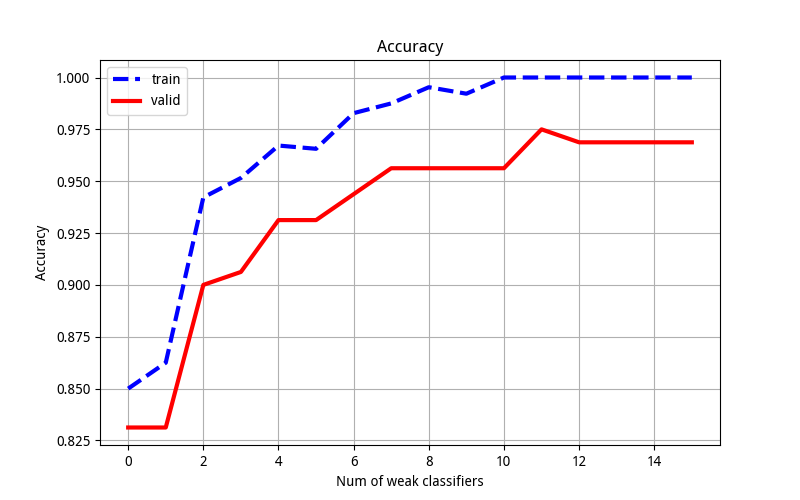
\includegraphics[width=\columnwidth]{../images/AdaBoost-accuracy.png}
        \end{center}
    \end{figure}
  
    The learning curve is very smooth, which means that the boosting process meets the requirements of this lab. As weak classifiers added, the accuracy gets much higher.

\section{Conclusion}
	This experiment is much more interesting than the past experiments. With slides provided by Mr. Wu, it is much easier to understand details of AdaBoost algorithm. 

% Your document ends here!
\end{document}